\documentclass[12pt]{article}

\usepackage{sbc-template}
\usepackage{graphicx,url}
\usepackage[utf8]{inputenc}
\usepackage[brazil]{babel}
\usepackage[latin1]{inputenc}  

     
\sloppy

\title{Simulated Annealing\\ Uma resolução para SAT-3}

\author{César Eduardo de Souza\inst{1},\\ Guilherme Diel\inst{1}}


  \address{Departamento de Ciência da Computação \\ Universidade do Estado de Santa Catarina
  (UDESC) -- Joinville, SC -- Brazil
  \email{\{cesar.souza, guilherme.diel\}@edu.udesc.br}
}

\begin{document} 

\maketitle

\begin{abstract}
  Abstract
\end{abstract}
     
\begin{resumo} 
  Resumo
\end{resumo}


\section{Introdução}
% Contextualização do problema/tarefa e revisão da literatura.

Foi no século XX que se iniciou a busca pela resolução de problemas NP, NP-Hard e NP-Completo usando ferramentas computacionais. 
%
Estas portanto, foram, em sua maioria, desenvolvidos com base em algoritmos heurísticos – alicerçados em técnicas de busca de solução não necessariamente ótima, mas sim satisfatória –. 
%
Sendo assim, alguns destes tornaram-se mais disseminados na literatura científica, como a \textbf{Busca Gulosa}, \textbf{Algoritmo A*}, \textbf{Subida de Encosta} e \textbf{Simulated Annealing}. 

O método de \textbf{Simulated Annealing} teve sua lógica concebida a partir do método de anelização de materiais, Metropolis, desenvolvido por Gibbs em 1953 \cite{Gibbs}.
%
Basado na fabricação de aneis, este método usa como base o fato de que, quanto mais quente está o material, maior se torna a facilidade de modelá-lo.
%
Sob o mesmo ponto de vista, este método consiste em uma sequencia de temperaturas decrescentes em que, quanto maior a temperatura atual, mais aleatorizada são as otimizações geradas pelo algoritmo, sendo que, quando a temperatura chegar a um certo ponto idealizando a otimização do resultado conforme decresce a temperatura, até que esta se torne mínima.

Um problema muito conhecido e discutido na literatura, que é capaz de ser resolvido por algoritmos heuristicos, é o problema da satisfabilidade (SAT), que consiste em, dado um conjunto de cláusulas disjuntivas na forma normal conjuntiva, determinar se existe uma atribuição de valores lógicos (\textit{verdadeiro} ou \textit{falso}) às variáveis envolvidas que satisfaça toda a expressão.
%
Cada cláusula é composta por uma disjunção (operador lógico $\lor$) de literais (variáveis ou suas negações), e a fórmula booleana global é uma conjunção (operador lógico $\land$) dessas cláusulas. Formalmente:

\begin{equation}
\bigwedge_{i=1}^{m} \left( \bigvee_{j=1}^{k} l_{ij} \right)
\end{equation}

Ao longo deste relatório, será abordado uma proposta de implementação de do \textbf{Simulated Annealing} para resolução de uma variante do SAT, conhecido como SAT-3, que consiste em três variáveis por cláusula no problema SAT.

Este relatório está organizado da seguinte maneira: a seção 2 apresenta estratégias utilizadas, descrições, justificativas de escolhas, fórmulas utilizadas e descrições. Em seguida, na seção 3 são abordadas descrições dos experimentos, configurações utilizadas e descrições dos resultados obtidos. Outrossim, na seção 4 expõem-se considerações sobre os resultados obtidos e análises críticas sobre os mesmos. Por fim, na seção 5 mostra-se considerações sobre o trabalho desenvolvido e identificação de direcionamentos futuros na pesquisa.


% Justificativa e motivação.
% Objetivo.
% Organização do texto.

\section{Metodologia de Desenvolvimento} \label{sec:firstpage}

O método de \textbf{Simulated Annealing} consiste em:
\begin{enumerate}
  
  \item Para uma temperatura $T_i$, realizar $N$ vezes: \label{passo:1}
  \begin{itemize}
    \item Realizar uma perturbação aleatória no estado atual $\text{estado}_0$, gerando um novo $\text{estado}_i$
    \item Calcular a variação de energia $\Delta E = E(\text{estado}_i) - E(\text{estado}_0)$
    \item Se $\Delta E < 0$ (melhora na energia), aceitar a transição ($\text{estado}_i \rightarrow \text{estado}_0$)
    \item Caso contrário, aceitar a transição com probabilidade P_{\text{accept}}($T_i$)
  \end{itemize}
  
  \item Critério de parada:
  \begin{itemize}
    \item Se $T_i \leq T_f$ (temperatura final) ou o sistema atingir convergência (e.g., $\Delta E \approx 0$ por $k$ iterações consecutivas)
    \item Retornar o $\text{estado}_0$ como solução
    \item Caso contrário, reduzir a temperatura ($T_i \leftarrow \alpha T_i$, com $0 < \alpha < 1$) e retornar ao Passo~\ref{passo:1}
  \end{itemize}
  \label{pseudocodigo}
  \caption{Passo a passo do método de \textbf{Simulated Annealing}}
\end{enumerate} 

A aplicação do método de \textbf{Simulated Annealing} para a otimização do problema do SAT-3 foi realizada por meio da linguagem de programação \textit{Python}, junto com a biblioteca \textit{Numpy}.
%
A Figura \ref{fig:metodologia} retrata o passo a passo de como foi implementado este algoritmo.
%
O passo 1 (inicialização) consiste em realizar a inicialização do sistema:

\begin{itemize}
  \item Temperatura inicial $T_0$ = 1000
  \item Taxa de resfriamento \alpha = 0.99
  \item Temperatura final $T_f$ = 0.1
  \item Número de iterações por temperatura $N$ = 1000
\end{itemize}

No segundo passo (iteração por temperatura) da Figura \ref{fig:metodologia} a fórmula de probabilidade de aceitação de estados com pior energia que foi adotada, foi:
\begin{equation}
  P_{\text{accept}} = \exp\left(-\frac{\Delta E}{T_i}\right)
\end{equation}

O terceiro passo (resfriamento) corresponde ao passo \ref{passo:1} do codigo de \ref{pseudocodigo}.

\begin{figure}[ht]
  \centering
  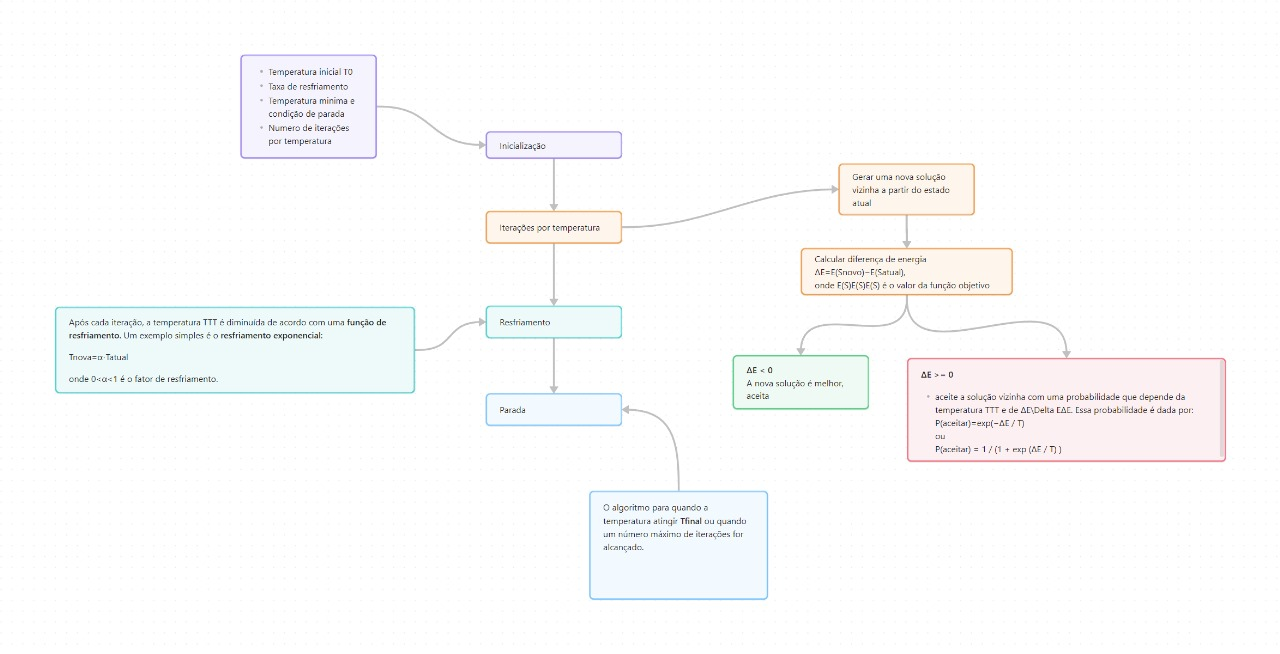
\includegraphics[width=1\textwidth]{pasta_.jpeg}
  \caption{A typical figure}
  \label{fig:metodologia}
  \end{figure}
% descrições e justificativas das escolhas.
% Fórmulas utilizadas, descrições e justificativas.

\section{Descrição de Experimentos/Simulações e Resultados Obtidos}

% Descrição dos experimentos
% e configurações utilizadas.

Foi com a temperatura inicial = 1000 = iterações por temperatura taa de resfriamento = 0.99 
que foram obtidos os resultados para a média de 30 execuções

% Descrição dos resultados obtidos (Figuras, Tabelas, Gráficos).

Nestas configurações foram obtidos resultados para bases de SAT-3 de 20, 100 e 250 entradas % to pensando em fazer o \ref pra cada um mas sla tb

\begin{figure}[ht!]
  \centering
  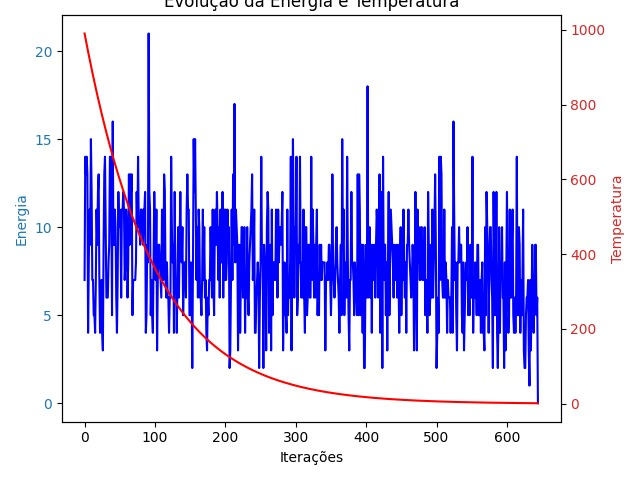
\includegraphics[width=.5\textwidth]{20_entries_plot.jpg}
  \caption{20 Entradas}
  \label{fig:metodologia}
  \end{figure}

\begin{figure}[ht!]
  \centering
  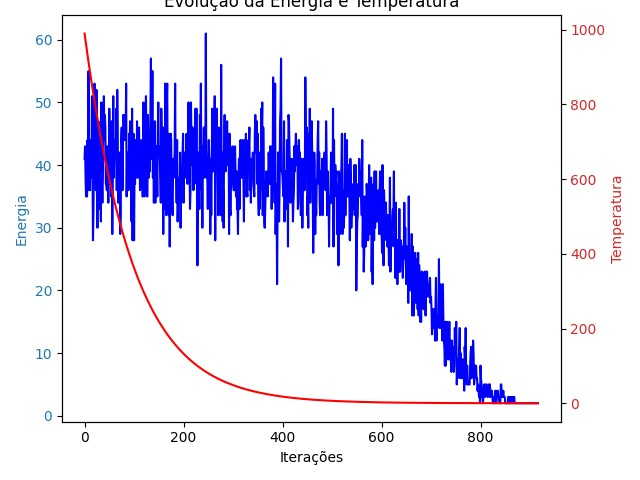
\includegraphics[width=.5\textwidth]{100_entries_plot.jpg}
  \caption{100 Entradas}
  \label{fig:metodologia}
   \end{figure}

\begin{figure}[ht!]
  \centering
  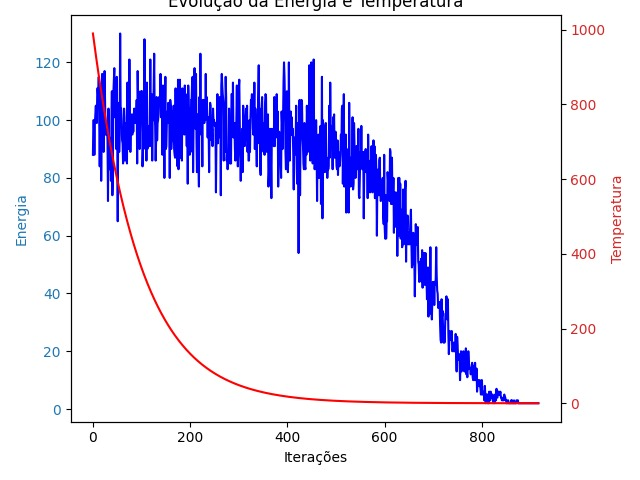
\includegraphics[width=.5\textwidth]{250_entries_plot.jpg}
  \caption{250 Entradas}
  \label{fig:metodologia}
  \end{figure}


\section{Análise dos resultados obtidos.}

Considerações sobre os resultados obtidos e análises críticas sobre os mesmos.

\section{Conclusões e Trabalhos Futuros}\label{sec:figs}


Considerações sobre o trabalho desenvolvidos e identificação de direcionamentos futuros na
pesquisa.



\bibliographystyle{sbc}
\bibliography{sbc-template}

\end{document}
